\documentclass{beamer}
\usetheme[pageofpages=of,% String used between the current page and the
                         % total page count.
          bullet=circle,% Use circles instead of squares for bullets.
          titleline=true,% Show a line below the frame title.
          alternativetitlepage=true,% Use the fancy title page.
       %   titlepagelogo=logo-polito,% Logo for the first page.
       %   watermark=watermark-polito,% Watermark used in every page.
       %   watermarkheight=100px,% Height of the watermark.
       %   watermarkheightmult=4,% The watermark image is 4 times bigger
                                % than watermarkheight.
          ]{Torino}

\setbeamertemplate{footline}{
  \begin{beamercolorbox}[wd=\paperwidth,ht=1ex,dp=1ex]{footline}
    \vspace{5pt} \hspace{1em} \insertframenumber/\inserttotalframenumber
  \end{beamercolorbox}
}

\author{Brendon J. Brewer}
\title{STATS 331 -- Introduction to Bayesian Statistics}
\institute{The University of Auckland}
\date{}


\linespread{1.3}
\usepackage{minted}
\usepackage[utf8]{inputenc}
\usepackage{dsfont}
\newcommand{\given}{\,|\,}

\begin{document}

\frame{\titlepage}

\begin{frame}
\begin{center}
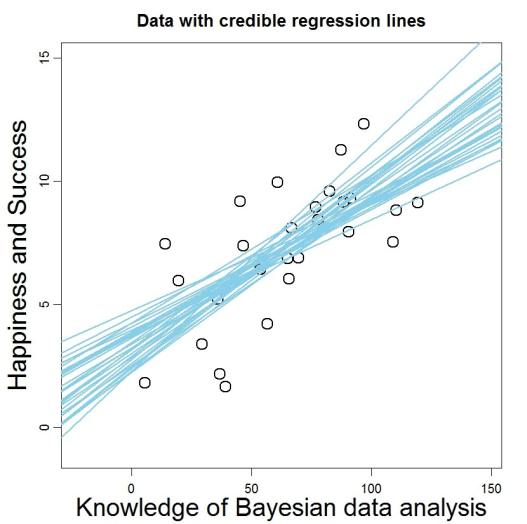
\includegraphics[width=0.6\textwidth]{images/happiness.png} \\
Credit: John Kruschke
\end{center}

\end{frame}


\begin{frame}
\frametitle{Plan}
\begin{itemize}
\item We will now look at two examples of Bayesian parameter estimation,
one of which also involves a {\bf prediction}.\pause
\item In both cases, we'll get the likelihood by defining the
{\bf sampling distribution} first.\pause
\item We will introduce a different ``non-informative'' prior distribution
that isn't uniform.
\end{itemize}

\end{frame}


\begin{frame}
\frametitle{Reminder of Bayes' Rule for Parameter Estimation}

\begin{align}
p(\theta \given x) &= \frac{p(\theta)p(x \given \theta)}{p(x)} \\
p(\theta \given x) &\propto p(\theta)p(x \given \theta) \\
\texttt{posterior} &\propto \texttt{prior} \times \texttt{likelihood}
\end{align}
(notation: $\theta$=parameter, $x$=data)

\end{frame}



\begin{frame}
\frametitle{Taxi Problem}

    \begin{columns} % Create two columns
        \column{0.5\textwidth} % Left column (50% width)

        \begin{itemize}
        \item You fall asleep in a foreign city.
        \item When you wake up in the morning, you see a taxi drive by,
              which says {\bf This is taxi number 42}.
        \item How many taxis are in the city?
        \end{itemize}

        \column{0.5\textwidth} % Right column (50% width)
        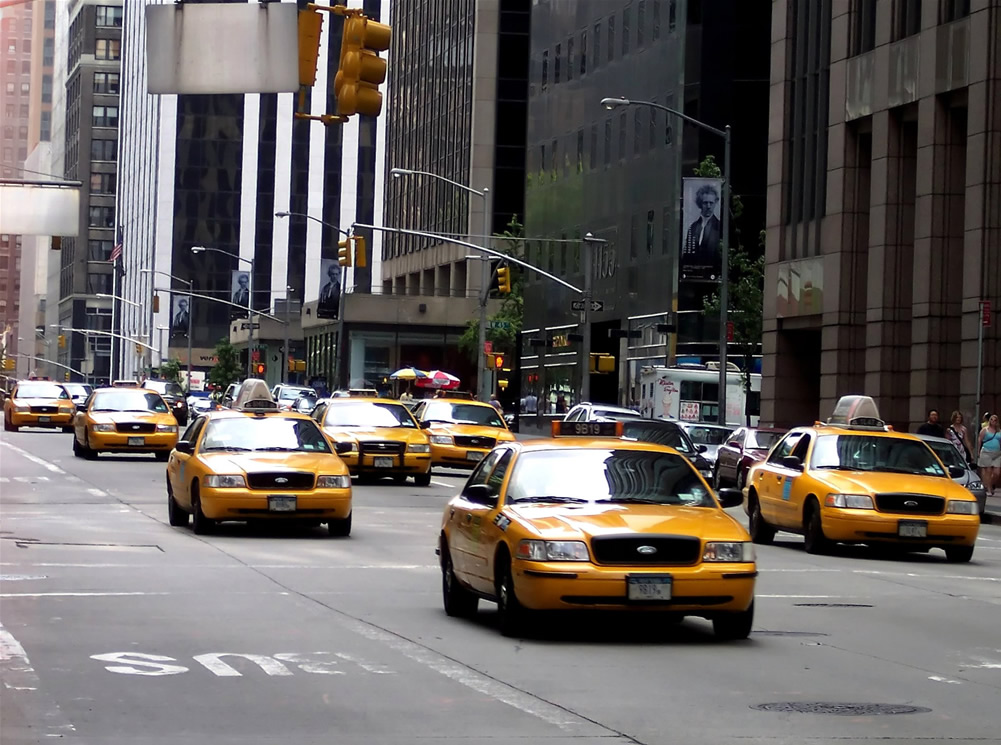
\includegraphics[width=0.95\linewidth]{images/taxis.jpg}
       
         (public domain image)
     \end{columns}

\end{frame}

\begin{frame}
\frametitle{The Parameter and the Data}

\begin{itemize}
\item The unknown parameter, $N$, is the number of taxis in the city.\pause
\item The data, $x$, is the number observed on the taxi that drove past.
\end{itemize}
\pause
Bayes' rule for this circumstance:

\begin{align}
p(N \given x) \propto p(N)p(x \given N)
\end{align}
We have to choose the prior $p(N)$ and the likelihood $p(x \given N)$.

\end{frame}


\end{document}

